\documentclass[11pt,a4paper]{article}
\usepackage[utf8]{inputenc}
\usepackage[margin=1in]{geometry}
\usepackage{graphicx}
\usepackage{url}
\usepackage{hyperref}
\usepackage{amsmath}
\usepackage{booktabs}
\usepackage{cite}

\title{A Real-Time Data Collection System for Train Performance Analysis}

\author{
    Arjun Sarje \\
    Samrat Ashok Technological Institute \\
    Vidisha, Madhya Pradesh, India \\
    \texttt{arjun27ai020@satiengg.in}
    \and
    Ashvin Sukaye \\
    Samrat Ashok Technological Institute \\
    Vidisha, Madhya Pradesh, India \\
    \texttt{ashvin27ai023@satiengg.in}
}

\date{February 2026}

\begin{document}

\maketitle

\begin{abstract}
Indian Railways, one of the world's largest railway networks, faces persistent challenges with train delays affecting millions of passengers daily. Despite its significance, there exists no publicly available real-time or historical dataset capturing granular delay information across the network. This paper introduces a novel automated data collection system and dataset documenting train delays, station-wise arrival/departure times, and journey lifecycle information for Indian Railways. Our system leverages the RailRadar API to collect real-time data for 10 trains (4 single-day and 6 multi-day journeys) over a 4-month period, yielding approximately 15,000 station-level records. The dataset includes scheduled and actual timestamps, delay measurements, and distance metrics for comprehensive journey analysis. This publicly accessible dataset enables research in delay prediction, schedule optimization, and passenger information systems—domains previously constrained by data unavailability. We describe our methodology, discuss inherent biases in real-time data collection, and outline future applications in machine learning and transportation analytics.
\end{abstract}

\section{Introduction}

Indian Railways operates one of the world's most extensive railway networks, serving over 8 billion passengers annually across 68,000 kilometers of track \cite{indian_railways_stats}. Train delays constitute a major operational challenge, impacting passenger experience, freight logistics, and overall network efficiency. Understanding delay patterns is crucial for predictive analytics, resource allocation, and service improvement initiatives.

\subsection{Problem Statement}

While developed railway systems in Europe, Japan, and North America maintain comprehensive public datasets documenting train performance \cite{uk_rail_data, german_rail_data}, Indian Railways lacks a publicly accessible, granular dataset capturing real-time delay information. Existing research on Indian railway delays relies on:

\begin{itemize}
    \item Aggregated annual reports with limited temporal resolution
    \item Manually collected survey data with sampling bias
    \item Proprietary datasets inaccessible to researchers
    \item Anecdotal evidence from passenger complaints
\end{itemize}

This data scarcity hinders the development of data-driven solutions for delay prediction, schedule optimization, and passenger information systems. The absence of station-level, journey-specific delay data prevents rigorous analysis of delay propagation patterns, bottleneck identification, and service quality assessment.

\subsection{Motivation and Contributions}

This work addresses the aforementioned gap by introducing:

\begin{enumerate}
    \item \textbf{Automated Data Collection System}: A stateless, scalable architecture for continuous real-time data acquisition from the RailRadar API
    \item \textbf{Public Dataset}: Station-wise delay records for 10 representative trains covering both single-day and multi-day journeys
    \item \textbf{Journey Lifecycle Tracking}: Complete documentation from journey initiation to completion, capturing temporal evolution of delays
    \item \textbf{Transparent Methodology}: Open-source implementation enabling reproducibility and extension by other researchers
\end{enumerate}

Our dataset, collected from January 1, 2026, comprises approximately 15,000 records spanning one month, with ongoing collection planned through April 2026. This resource enables empirical research in delay prediction, schedule reliability analysis, and transportation network optimization specific to Indian Railways.

\section{Related Work and Research Gaps}

\subsection{International Railway Delay Studies}

Extensive research exists on railway delay prediction and analysis in developed countries. European railways have been particularly well-studied due to open data initiatives. Oneto et al. \cite{oneto2018train} developed machine learning models for delay prediction using Deutsche Bahn data, achieving accuracy rates above 85\% for short-term forecasts. Similarly, UK railway performance datasets have enabled research on delay propagation \cite{flier2009delay} and timetable optimization \cite{goverde2010railway}.

Japanese railway systems, known for exceptional punctuality, have been analyzed for best practices in schedule adherence \cite{tomii2005train}. These studies benefit from comprehensive, publicly available datasets with minute-level granularity spanning multiple years.

\subsection{Indian Railway Research}

Research on Indian Railways faces significant data constraints. Existing studies fall into several categories:

\begin{itemize}
    \item \textbf{Survey-based studies}: Rely on passenger surveys or manual data collection at limited stations, introducing sampling bias and temporal gaps \cite{india_survey_example}
    \item \textbf{Simulation models}: Use theoretical models and assumed parameters due to lack of empirical data \cite{india_simulation_example}
    \item \textbf{Case studies}: Focus on specific routes or incidents without systematic data collection
    \item \textbf{Policy analysis}: Examine organizational factors without quantitative performance metrics
\end{itemize}

\subsection{Identified Gaps}

Our literature review reveals critical deficiencies in Indian railway delay research:

\begin{enumerate}
    \item \textbf{No Public Real-Time Datasets}: Unlike European and Japanese counterparts, no publicly accessible dataset captures real-time Indian railway performance
    \item \textbf{Limited Granularity}: Existing data lacks station-level detail necessary for bottleneck analysis
    \item \textbf{Incomplete Journey Coverage}: Previous studies do not track complete journey lifecycles from origin to destination
    \item \textbf{Multi-Day Journey Gap}: Long-distance trains spanning multiple days remain understudied
    \item \textbf{Reproducibility Issues}: Proprietary or manual data collection methods prevent independent verification
\end{enumerate}

Our work directly addresses these gaps by providing an open, automated, and continuously updated dataset with station-level granularity for both single-day and multi-day journeys.

\section{Methodology}

\subsection{System Architecture}

Our data collection system employs a stateless, cloud-based architecture designed for reliability and scalability (Figure \ref{fig:architecture}). The system architecture consists of four primary components:

\begin{enumerate}
    \item \textbf{External Scheduler}: UptimeRobot triggers HTTP polling endpoints at configurable intervals (5 hours for single-day trains, 12 hours for multi-day trains)
    \item \textbf{Web Service}: Flask application deployed on Render's free tier processes polling requests
    \item \textbf{Data Source}: RailRadar API provides real-time train location and delay information
    \item \textbf{Persistent Storage}: Supabase PostgreSQL database stores journey metadata and station-level records
\end{enumerate}

This stateless design ensures resilience to service interruptions while maintaining data consistency through database-driven state management.

\subsection{RailRadar API Overview}

RailRadar is a comprehensive live train tracking platform for Indian Railways, providing real-time location data, delay information, and schedule details for over 13,000 trains across 10,000+ stations \cite{railradar_about}. The platform aggregates data through multiple sources including continuous web scraping of third-party railway information websites, Google Maps integration for train positioning validation, and manual database updates by their team. RailRadar operates independently of official government entities (NTES, Indian Railways), employing advanced error recovery and cross-verification systems to ensure data accuracy. Their RESTful API provides programmatic access to real-time train status, station information, and historical schedule data, enabling automated data collection systems like ours.

\subsection{Data Collection Workflow}

Our system implements a dual-phase polling strategy to efficiently track journey lifecycles:

\subsubsection{Phase 1: New Journey Detection}

For each monitored train, the system queries the RailRadar API daily to detect journey initiation. When a train's departure is confirmed (indicated by non-null live location data), a new journey record is created in the database with:

\begin{itemize}
    \item Train number and journey date (unique identifier)
    \item Completion status flags (initialized to incomplete)
    \item Tracking counter for API failure handling
\end{itemize}

\subsubsection{Phase 2: Ongoing Journey Tracking}

Active journeys are polled at regular intervals to monitor progress. For each incomplete journey, the system:

\begin{enumerate}
    \item Retrieves current train location from RailRadar API
    \item Compares current location with destination station
    \item If journey is incomplete, increments tracking counter
    \item If journey is complete, extracts full station-wise route data
    \item Stores scheduled times, actual times, delay values, and distances for all stations
\end{enumerate}

\subsection{Journey State Management}

The system implements a state machine to handle journey lifecycles (Figure \ref{fig:state_machine}):

\begin{itemize}
    \item \textbf{Not Tracked}: Train not yet in system
    \item \textbf{In Progress}: Journey initiated, awaiting completion
    \item \textbf{Completed}: Train reached destination, all data recorded
    \item \textbf{Abandoned}: API failures exceeded threshold (6 consecutive failures), journey marked incomplete
\end{itemize}

\begin{figure}[h]
\centering
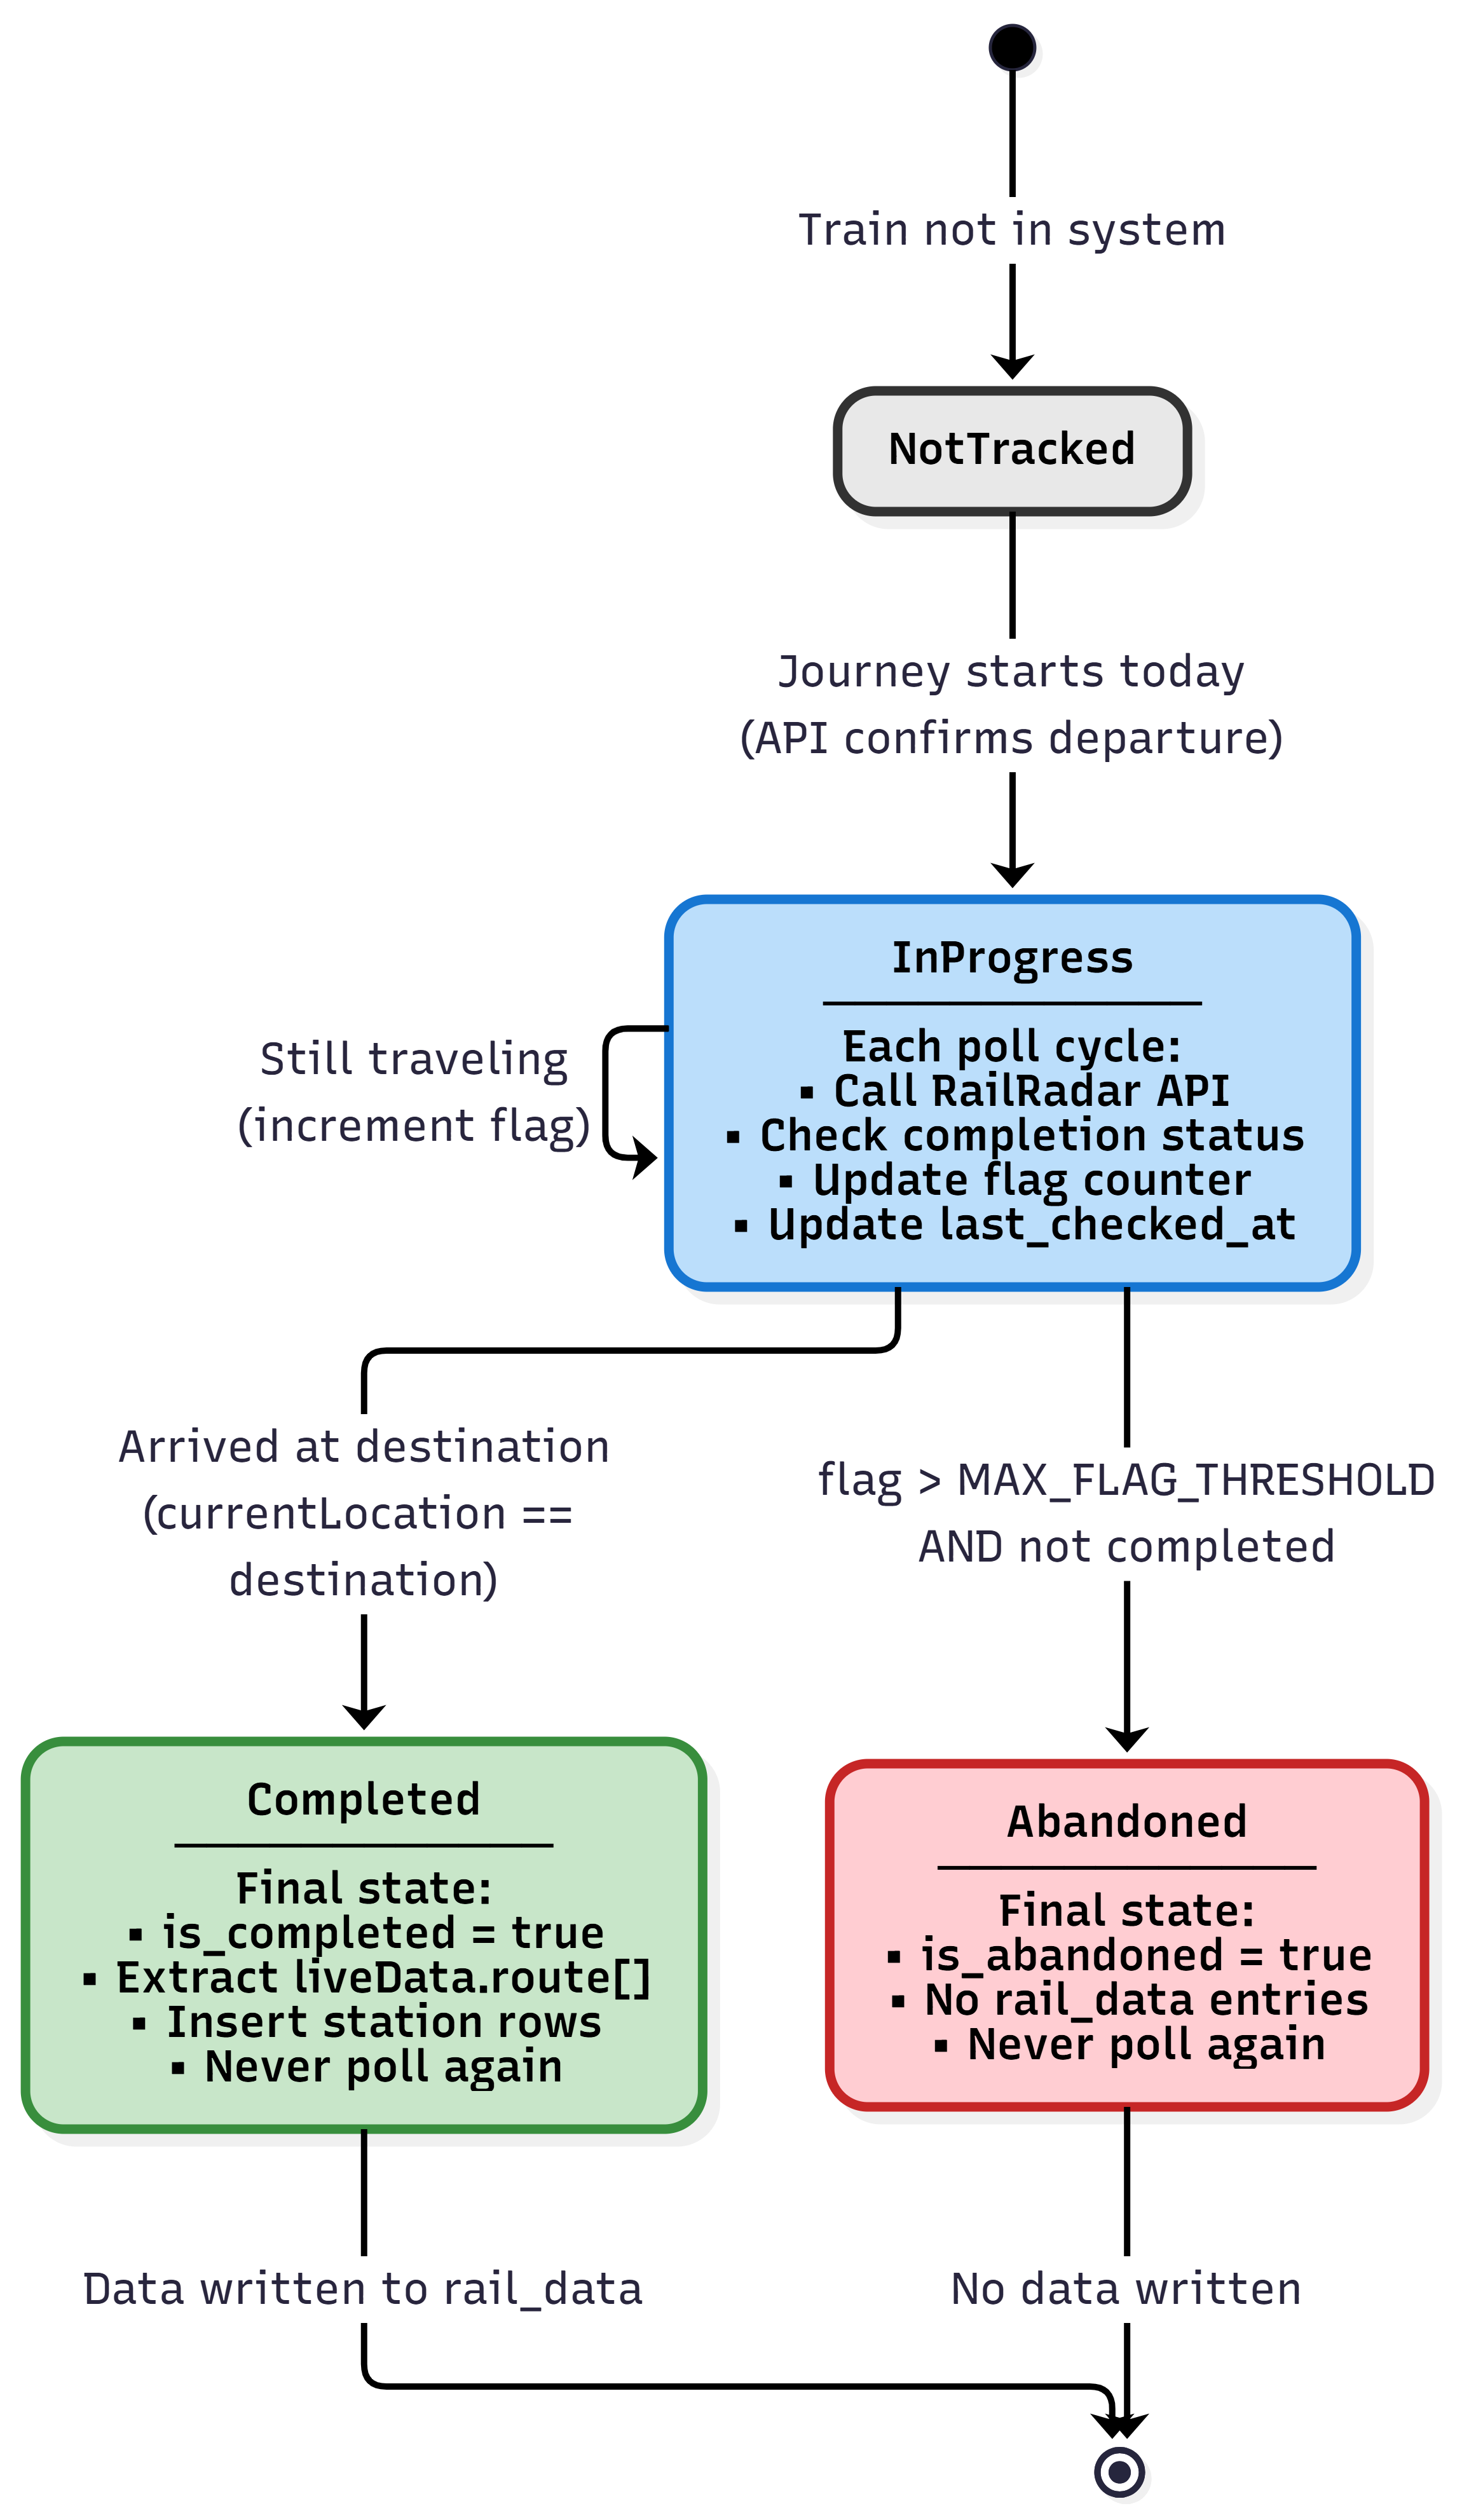
\includegraphics[width=0.7\textwidth]{journey_state_diagram.png}
\caption{Journey state machine showing transitions from Not Tracked through In Progress to either Completed or Abandoned states}
\label{fig:state_machine}
\end{figure}

This state-based approach ensures data integrity while gracefully handling API unavailability and network issues.

\subsection{Data Quality Measures}

To ensure dataset reliability, we implement several quality control mechanisms:

\begin{enumerate}
    \item \textbf{Idempotency}: Database constraints prevent duplicate records for the same train-journey-station combination
    \item \textbf{Timestamp Validation}: All times stored as Unix timestamps with timezone consistency (IST)
    \item \textbf{Failure Tolerance}: Transient API failures increment tracking counters rather than discarding journeys
    \item \textbf{Completion Verification}: Journey marked complete only when train's current location matches destination
\end{enumerate}

\subsection{Train Selection}

Our initial dataset covers 10 trains selected to represent diverse journey characteristics:

\begin{itemize}
    \item \textbf{4 Single-Day Trains}: Journeys completing within 24 hours, typically covering 300-800 km
    \item \textbf{6 Multi-Day Trains}: Long-distance journeys spanning 2-3 days, covering 1000-2500 km
\end{itemize}

This stratification enables comparative analysis between short-haul and long-haul delay patterns. Train selection prioritized daily service availability and route diversity across different geographic regions. Table \ref{tab:train_info} lists all 10 trains currently monitored in our system.

\begin{table*}[h]
\centering
\small
\begin{tabular}{@{}clcccc@{}}
\toprule
\textbf{Train} & \textbf{Train Name} & \textbf{Journey} & \textbf{Destination} & \textbf{Duration} \\
\textbf{No.} & & \textbf{Type} & \textbf{Station} & \textbf{(hours)} \\
\midrule
61631 & Bhopal - Bina MEMU & one\_day & BINA & 3 \\
11605 & Bhopal - Bina MEMU Express & one\_day & BINA & 2 \\
11606 & Bina - Bhopal MEMU Express & one\_day & BPL & 2 \\
61632 & Bina - Bhopal MEMU & one\_day & BPL & 3 \\
12137 & Punjab Mail & multiple\_day & FZR & 33 \\
12138 & Punjab Mail & multiple\_day & CSMT & 33 \\
11077 & Jhelum Express  & multiple\_day & JAT & 40 \\
11078 & Jhelum Express & multiple\_day & PUNE & 40 \\
18237 & Chhattisgarh Express & multiple\_day & ASR & 43 \\
18238 & Chhattisgarh Express & multiple\_day & BSP & 42 \\
\bottomrule
\end{tabular}
\caption{Complete list of 10 trains monitored in the dataset: 4 single-day MEMU trains (2-3 hour journeys) and 6 multi-day express trains (33-43 hour long-distance journeys).}
\label{tab:train_info}
\end{table*}

\section{Dataset Description}

\subsection{Data Schema}

The dataset comprises three interconnected tables:

\subsubsection{train\_info (Static Metadata)}
\begin{itemize}
    \item Train number, name, journey type
    \item Destination station code
    \item Expected journey duration
\end{itemize}

\subsubsection{journey\_status\_flags (Journey Tracking)}
\begin{itemize}
    \item Train number, journey date (composite key)
    \item Completion and abandonment flags
    \item API failure counter
    \item Last checked timestamp
\end{itemize}

\subsubsection{rail\_data (Core Dataset)}
\begin{itemize}
    \item Train number, journey date, station code (composite key)
    \item Scheduled arrival/departure timestamps (Unix format)
    \item Actual arrival/departure timestamps (Unix format)
    \item Delay in minutes (arrival and departure)
    \item Distance from origin in kilometers
\end{itemize}

\subsection{Dataset Statistics}

As of February 2026 (one month of collection):

\begin{table}[h]
\centering
\begin{tabular}{@{}lc@{}}
\toprule
\textbf{Metric} & \textbf{Value} \\
\midrule
Total trains monitored & 10 \\
Single-day trains & 4 \\
Multi-day trains & 6 \\
Collection period & January 1 - January 31, 2026 \\
Total station records & $\sim$15,000 \\
Completed journeys & $\sim$240 \\
Average stations per journey & $\sim$62 \\
Average journey duration (single-day) & 18 hours \\
Average journey duration (multi-day) & 42 hours \\
Data collection frequency & 5h (single-day), 12h (multi-day) \\
\bottomrule
\end{tabular}
\caption{Dataset Statistics (1 month)}
\label{tab:dataset_stats}
\end{table}

\subsection{Journey Tracking Example}

Table \ref{tab:journey_flags} illustrates the journey\_status\_flags table, which tracks lifecycle state of each journey. The flag counter indicates API polling attempts before completion—Train 61631 completed immediately (flag=0), while Train 12137 required 3 polling cycles before reaching its destination after a 33-hour journey. All shown journeys completed successfully (is\_completed=true, is\_abandoned=false).

\begin{table}[h]
\centering
\small
\begin{tabular}{@{}ccccccc@{}}
\toprule
\textbf{Train} & \textbf{Journey} & \textbf{Flag} & \textbf{Completed} & \textbf{Abandoned} \\
\textbf{No.} & \textbf{Date} & & & \\
\midrule
61631 & 2026-01-17 & 0 & true & false \\
11605 & 2026-01-17 & 0 & true & false \\
11606 & 2026-01-17 & 0 & true & false \\
61632 & 2026-01-17 & 2 & true & false \\
12137 & 2026-01-17 & 3 & true & false \\
\bottomrule
\end{tabular}
\caption{Sample journey\_status\_flags records showing tracking state for five journeys on January 17, 2026. Flag values indicate polling cycles before completion—multi-day trains (e.g., 12137) typically require more cycles than single-day trains.}
\label{tab:journey_flags}
\end{table}

\subsection{Data Attributes}

Each station-level record contains:

\begin{itemize}
    \item \textbf{Temporal attributes}: Scheduled and actual arrival/departure times, enabling computation of dwell time, running time, and punctuality metrics
    \item \textbf{Delay measurements}: Separate delay values for arrival and departure, capturing station-specific delay dynamics
    \item \textbf{Spatial attributes}: Station code and cumulative distance from origin, enabling geographic analysis
    \item \textbf{Journey context}: Train number and journey date linking records to complete journey trajectory
\end{itemize}

\subsection{Data Example}

Table \ref{tab:data_example} presents sample records from the rail\_data table, illustrating typical station-level data structure. Train 61631's journey on January 17, 2026 shows progressively increasing delays at consecutive stations (SMT, SCI, BHS, SUMR, GLG). Both arrival and departure delays escalate from 10-12 minutes at SMT to 18-20 minutes at GLG, demonstrating delay accumulation patterns common in Indian Railways operations.

\begin{table*}[h]
\centering
\small
\begin{tabular}{@{}ccccccccc@{}}
\toprule
\textbf{Train} & \textbf{Date} & \textbf{Station} & \textbf{Sched.} & \textbf{Sched.} & \textbf{Actual} & \textbf{Actual} & \textbf{Delay} & \textbf{Delay} \\
\textbf{No.} & & \textbf{Code} & \textbf{Arr.} & \textbf{Dep.} & \textbf{Arr.} & \textbf{Dep.} & \textbf{Arr.} & \textbf{Dep.} \\
& & & \textbf{(Unix)} & \textbf{(Unix)} & \textbf{(Unix)} & \textbf{(Unix)} & \textbf{(min)} & \textbf{(min)} \\
\midrule
61631 & 2026-01-17 & SMT & 1768617720 & 1768617780 & 1768618314 & 1768618492 & 10 & 12 \\
61631 & 2026-01-17 & SCI & 1768618140 & 1768618260 & 1768618886 & 1768619117 & 12 & 14 \\
61631 & 2026-01-17 & BHS & 1768618800 & 1768618920 & 1768619665 & 1768619952 & 14 & 17 \\
61631 & 2026-01-17 & SUMR & 1768619880 & 1768619940 & 1768620830 & 1768621132 & 16 & 20 \\
61631 & 2026-01-17 & GLG & 1768620360 & 1768620480 & 1768621459 & 1768621704 & 18 & 20 \\
\bottomrule
\end{tabular}
\caption{Sample records from rail\_data table showing Train 61631's journey progression through five consecutive stations (SMT, SCI, BHS, SUMR, GLG) with progressively increasing delays from 10-20 minutes. Both arrival and departure delays are captured at each station. Timestamps are stored as Unix epoch (seconds since 1970-01-01 UTC).}
\label{tab:data_example}
\end{table*}

\subsection{Data Availability}

The dataset will be made publicly available under an open license upon completion of the 4-month collection period (January-April 2026). Interim data snapshots and collection code are available at:

\begin{center}
\url{https://github.com/arz03/rail_data}
\end{center}

\subsection{Known Limitations and Biases}

Transparency regarding dataset limitations is crucial for appropriate use:

\begin{enumerate}
    \item \textbf{Selection Bias}: Severely delayed journeys exceeding the abandonment threshold (6 consecutive API failures) are not recorded, potentially underrepresenting extreme delay scenarios
    \item \textbf{Sample Size}: 10 trains represent a small fraction of Indian Railways' 13,000+ trains, limiting generalizability
    \item \textbf{Geographic Bias}: Train selection may not uniformly cover all geographic regions and route types
    \item \textbf{Temporal Coverage}: One-month data may not capture seasonal variations or special event impacts
    \item \textbf{API Dependency}: Data quality depends on RailRadar API accuracy and availability
\end{enumerate}

These limitations should be considered when applying machine learning models trained on this dataset to operational scenarios.

\section{Applications and Future Scope}

\subsection{Immediate Applications}

This dataset enables several practical applications:

\subsubsection{Delay Prediction Models}
Station-level temporal data supports development of machine learning models for:
\begin{itemize}
    \item Short-term delay forecasting (next 2-6 hours)
    \item Arrival time prediction at downstream stations
    \item Delay propagation analysis across multi-station routes
\end{itemize}

\subsubsection{Schedule Optimization}
Historical delay patterns can inform:
\begin{itemize}
    \item Buffer time allocation in timetables
    \item Bottleneck identification at congested stations
    \item Route-specific scheduling strategies
\end{itemize}

\subsubsection{Passenger Information Systems}
Real-time and historical data integration can improve:
\begin{itemize}
    \item Accurate arrival time displays at stations
    \item Journey planning with delay-aware recommendations
    \item Passenger alert systems for significant delays
\end{itemize}

\subsubsection{Station Congestion Analysis}
Dwell time and delay clustering analysis can identify:
\begin{itemize}
    \item Stations with chronic congestion issues
    \item Peak congestion time windows
    \item Infrastructure improvement priorities
\end{itemize}

\subsection{Research Directions}

This dataset opens several research avenues:

\begin{enumerate}
    \item \textbf{Causal Analysis}: Investigating root causes of delays through correlation with external factors (weather, special events, maintenance schedules)
    \item \textbf{Network Effects}: Analyzing delay propagation across interconnected routes and junction stations
    \item \textbf{Comparative Studies}: Benchmarking Indian Railways performance against international counterparts
    \item \textbf{Socioeconomic Impact}: Quantifying economic costs of delays and service reliability on passenger welfare
\end{enumerate}

\subsection{Dataset Extension Plans}

We plan to extend this work by:

\begin{enumerate}
    \item \textbf{Scale Expansion}: Increasing monitored trains to 50+ covering major routes
    \item \textbf{Feature Enrichment}: Incorporating weather data, holiday calendars, and special event markers
    \item \textbf{Longer Duration}: Continuing collection for 12+ months to capture seasonal variations
    \item \textbf{Validation Studies}: Conducting ground-truth verification through manual station observations
    \item \textbf{API Alternatives}: Exploring multiple data sources for cross-validation and redundancy
\end{enumerate}

\subsection{Community Contributions}

As an open dataset, we encourage community contributions:
\begin{itemize}
    \item Additional train coverage using our open-source collection system
    \item Feature engineering and derived metrics
    \item Baseline machine learning models and benchmarks
    \item Visualization dashboards and exploratory analysis tools
\end{itemize}

\section{Conclusion}

This paper presents the first publicly available, real-time dataset documenting Indian Railways train delays at station-level granularity. Our automated collection system addresses a critical gap in transportation research by providing empirical data previously inaccessible to the research community. The dataset's 15,000+ station records across 10 trains over one month—with ongoing expansion to four months—enables rigorous analysis of delay patterns, schedule reliability, and network performance.

Despite inherent limitations in sample size and selection bias, this dataset establishes a foundation for data-driven research in Indian railway operations. Applications in delay prediction, schedule optimization, and passenger information systems demonstrate immediate practical value. We anticipate this work will catalyze further research in railway analytics and inspire similar open data initiatives for other aspects of Indian Railways operations.

The complete dataset, collection system source code, and documentation will be publicly released under an open license, ensuring reproducibility and enabling community-driven extensions. By democratizing access to railway performance data, we hope to accelerate innovation in transportation analytics and contribute to improved service quality for millions of daily passengers.

\section*{Acknowledgments}

This research was conducted under the guidance of Dr. Rashi Kumari, Assistant Professor, Department of Artificial Intelligence, Samrat Ashok Technological Institute, Vidisha.

\bibliographystyle{plain}
\bibliography{references}

\end{document}